\documentclass[french,12pt,a4paper]{book}

% headers and typo stuffs
\usepackage{fancyhdr}
\usepackage{array}
\usepackage{geometry}
\usepackage{multirow} %% Pour mettre un texte sur plusieurs rangées
\usepackage{multicol} %% Pour mettre un texte sur plusieurs colonnes
\usepackage{scrextend} %Forcer la 4eme  de couverture en page pair
\usepackage[utf8]{inputenc}
\usepackage[T1]{fontenc}
\usepackage{titlesec} % change titles formatting
\usepackage{tocloft} %% toc formatting
%\usepackage[french]{babel} % deactivating french babel that yields an error
%\usepackage{csquotes} % for csquotes not present in babel french
\usepackage[absolute]{textpos} 
\usepackage{lipsum}
% fonts
\usepackage{lmodern}
%---------------------------------------------------------
% Semi-bold condensed. Works only with lmodern
\def\sbc{\sffamily\fontseries{sbc}\selectfont}


\usepackage[dvipsnames]{xcolor} % colors
% links and url
\usepackage{hyperref}       % hyperlinks
\usepackage{url}            % simple URL typesetting
\hypersetup{%pdftex,  % needed for pdflatex
  breaklinks=true,  % so long urls are correctly broken across lines
  colorlinks=true,
  urlcolor=deep_brown,
  linkcolor=deep_blue,
  citecolor=dark_green,
  }

  \usepackage{enumitem}
  \setlist[itemize]{label=\textcolor{myblue}{\rule{1ex}{1ex}}}
  \setlist[description]{font=\bfseries\sffamily}
  \setlist[enumerate]{font=\bfseries\sffamily\color{myblue}}
  
  
% figures
\usepackage{graphicx}
\usepackage{caption}
\usepackage{subcaption}
\usepackage{placeins}
% tables
\usepackage{booktabs} % professional-quality tables
\usepackage{tabularx}
\usepackage{colortbl}
\usepackage{threeparttable}
\usepackage{multirow}
\usepackage{makecell}
% csv
\usepackage{csvsimple}
% maths
\usepackage{amsfonts}  % blackboard math symbols
\usepackage{amsmath}
\usepackage{amssymb} %mathbb packages

\usepackage{siunitx}
\usepackage{algorithm, algorithmicx, algpseudocode}
% TODO: test if not happy with current algo styling
%\usepackage[ruled, linesnumbered, fillcomment]{algorithm2e}

% color commands
\colorlet{P}{ForestGreen}
\colorlet{I}{MidnightBlue}
\colorlet{C}{YellowOrange}
\colorlet{O}{DarkOrchid}
\definecolor{Prune}{RGB}{99,0,60}
\definecolor{light_grey}{rgb}{0.3,.3,.3}
\definecolor{deep_blue}{rgb}{0,.2,.5}
\definecolor{dark_blue}{rgb}{0,.15,.5}
\definecolor{myblue}{rgb}{.01,0.21,0.71}
% Less saturation in the green for citations
\definecolor{dark_green}{rgb}{0.2,0.5,.3}
%\definecolor{dark_green}{rgb}{0,0.5,.15}
\definecolor{firebrick}{rgb}{0.75,0.125,0.125}
\definecolor{indigo}{rgb}{0.3,0,0.5}
% Color from http://paletton.com/#uid=30v0u0kllllaFw0g0qFqFg0w0aF
\definecolor{dark_brown}{RGB}{85, 39, 0}
\definecolor{deep_brown}{RGB}{128, 70, 21}
\definecolor{lightgreen}{RGB}{138,255,138}
\definecolor{lightblue}{RGB}{138,138,255}
\definecolor{lightorange}{RGB}{255,212,138}
\colorlet{deep_color}{deep_blue}
\colorlet{dark_color}{dark_blue}
\colorlet{mycolor}{myblue}
\colorlet{chaptercolor}{deep_blue}
 % strange need to upper case for section numbering
\colorlet{CHAPTERCOLOR}{chaptercolor}
\colorlet{GRAY}{Gray}

% bibliography
\usepackage[natbib=true,style=authoryear,maxnames=999,maxcitenames=2,backend=biber]{biblatex}
% separators for bib
\DeclareDelimFormat{finalnamedelim}{\addsemicolon\space}
\DeclareDelimFormat[bib]{nametitledelim}{\addcolon\space}
\DeclareDelimFormat[bib]{titleyeardelim}{\addcomma\space}
% color for citations
\DeclareFieldFormat{biblabelnumber}{\textcolor{dark_green}{#1}}
% small bibliography
\DeclareFieldFormat{bibfont}{\footnotesize\sloppy #1}
\addbibresource{../references.bib}

% appendix
\usepackage[toc,titletoc,page]{appendix}

% notes in the margin
\usepackage{todonotes}
\usepackage{snaptodo}

% comments
\snaptodoset{block rise=1em}
\snaptodoset{margin block/.style={font=\tiny}} \newcommand{\gv}[1]{%
  \snaptodo[margin block/.append style=green!50!black]{%
    \sloppy\textbf{Gael}: #1}}
\snaptodoset{margin block/.style={font=\tiny}} \newcommand{\md}[1]{%
  \snaptodo[margin block/.append style=blue]{%
    \sloppy\textbf{Matthieu}: #1}}

%%%%%%% boxes %%%%%%%%
\usepackage{tikz}
\usepackage{mdframed}
\usepackage[skins]{tcolorbox}

% Define a new box environment lefthandside background information box

\usepackage{environ}
\usepackage[%
  linewidth=2pt,
  linecolor=background_info_color,
  middlelinewidth=0.4pt,
  roundcorner=1pt,
  topline = false,
  rightline = false,
  bottomline = false,
  rightmargin=0pt,
  skipabove=0pt,
  skipbelow=0pt,
  leftmargin=-30pt,
  innerleftmargin=0pt,
  innerrightmargin=0pt,
  innertopmargin=0pt,
  innerbottommargin=0pt,
  usetwoside=false
  ]{mdframed}
  \newlength{\coloredrulerwidth}
\setlength{\coloredrulerwidth}{\dimexpr 1cm+\mdflength{innerleftmargin}}
  \NewEnviron{background_box_left}{%
  \begin{mdframed}
      \noindent\hspace*{\dimexpr -\mdflength{innerleftmargin}-\coloredrulerwidth}\rule[-\textheight]{\coloredrulerwidth}{\textheight}
      \hspace*{\dimexpr \coloredrulerwidth + 5pt} % Adjust the spacing between ruler and label
      \rotatebox[origin=c]{90}{\textit{HELLO}} % Rotate the label text vertically
      \BODY % Content of the environment
  \end{mdframed}
}

\tcbuselibrary{breakable}
\tcbset{%
  mytitle/.style={%
      enhanced,
      overlay={
          \node [rotate=90, anchor=south, fill=tcbcolframe!25] at (frame.west) {\itshape \scriptsize #1};
        },
    },
  rightrule=0pt,
  skin=enhanced,parbox=false,breakable
}
\colorlet{background_info_color}{green!10!orange}
\newtcolorbox{background_box_left_old}[1][]{
  mytitle=\textcolor{background_info_color}{Background Information},
  %title style={flushright},
  colframe=background_info_color, enhanced, colback=white, frame hidden, enlarge
  left by=-1cm,boxsep=0mm, left=1cm, borderline west =
    {2pt}{0pt}{background_info_color}, #1 }

% Define a new box environment for citations
\newenvironment{citationbox}{
  \begin{tcolorbox}[
      enhanced,
      colback=gray!10, % Background color of the box (gray with 10% intensity)
      colframe=white, % Border color of the box (white)
      arc=0mm, % Roundness of the corners (0mm means sharp corners)
      boxrule=0.5pt, % Border width (adjust as needed)
      rightrule=0pt, % Right border width (0pt for no border on the right side)
      %enlarge left by=8cm,
      left=0pt, % Left margin (0pt means no extra margin on the left)
      right=0pt, % Right margin (0pt means no extra margin on the right)
      top=0pt, % Top margin (0pt means no extra margin on the top)
      bottom=0pt, % Bottom margin (0pt means no extra margin on the bottom)
      rightupper=10mm, % Extra space on the right side for the citation
      rightlower=10mm, % Extra space on the right side for the citation
      %halign=flush right, % Text alignment within the box (right-aligned)
      width=0.7\textwidth,
      flush right
    ]
    }{
  \end{tcolorbox}
}
%Handling Keywords
\def\keywordname{{\bfseries \emph Keywords}}%
\def\keywords#1{\par\addvspace\medskipamount{\rightskip=0pt plus1cm
    \def\and{\ifhmode\unskip\nobreak\fi\ $\cdot$
    }\noindent\keywordname\enspace\ignorespaces#1\par}}


% equations commands
\newcommand{\indep}{\perp \!\!\! \perp}
\newtheorem{assumption}{Assumption}
\newtheorem{definition}{Definition}
\newtheorem{proposition}{Proposition}
\newtheorem{proposition*}{Proposition}
\newtheorem{lemma}{Lemma}
\newtheorem{proof}{Proof}

\DeclareMathOperator*{\argmin}{argmin} \def\mycitecolor{green!50!black}
\usepackage{mathtools}
\newcommand\myeq{\stackrel{\mathclap{\text{def}}}{=}}

%%%%%%%%%%%%% Styling for contents (chapter, title, caption, ...) %%%%%%%%%%%%

% Styling of section numbering to have the chapter number hang
% The color of the chapter number outside of the section titles
% The font of section numbers in titles
\let\fontnumber\relax
% A box to retrieve the width of section labels.
\newsavebox{\mysectionbox}
% Use it to offset titles in the display of sections

\renewcommand\thesection{\fontnumber{\color{chaptercolor}\arabic{chapter}.}\arabic{section}}
\renewcommand\thesubsection{\fontnumber{\color{chaptercolor}\arabic{chapter}.}\arabic{section}.\arabic{subsection}}

% Section fonts
\titleformat{\chapter}[display]
  {\Huge\sffamily\raggedright}
  {\chaptertitlename\ \thechapter}
  {20pt}
  {\Huge}

\titleformat{\section}
  {\Large\bfseries\sffamily}
  {\thesection}
  {1em}
  {}

\titleformat{\subsection}
  {\large\bfseries\sffamily}
  {\thesubsection}
  {1em}
  {}

\titleformat{\paragraph}
  {\bfseries}
  {}
  {0em}
  {}

% The caption

\DeclareCaptionFont{captionnamefont}{\small\sffamily\color{MidnightBlue}}
\DeclareCaptionFont{captiontitlefont}{\small\sffamily}

\captionsetup{
  font={captionnamefont,captiontitlefont},
  labelfont=bf,
  labelsep=period,
  format=plain,
  figurename=Fig.
}
% ------------------------------------------------------------------
% chapter color
\definecolor{ared}{rgb}{.647,.129,.149}

\titleformat{\chapter}[display]
  {\normalfont\Huge\bfseries\color{ared}}
  {\hfill \chaptertitlename\ \thechapter}
  {20pt}
  {\Huge\itshape\filleft}
  

% ------------------------------------------------------------------
% Table of content
\setcounter{tocdepth}{2}
\renewcommand{\cftchapfont}{\bfseries\sffamily}
\renewcommand{\cftsecfont}{\sffamily}
\renewcommand{\cftsubsecfont}{\small\sffamily}

% headers
\usepackage{lastpage}
\usepackage{textcase}

\fancypagestyle{basic}{%
  \fancyhf{} % Clear header and footer
  \fancyhead[R]{\small \sffamily \nouppercase{\rightmark}} % Display subsections in the head
  %\fancyhead{\scriptsize \sffamily\rightmark} % Clear header
  \fancyfoot[C]{} % Centered footer
  \fancyfoot[R]{\small\sffamily M. Doutreligne} % Right footer
  \fancyfoot[L]{\small \thepage\,/\,\protect\pageref*{LastPage}} % Left footer
}

% ------------------------------------------------------------------
% The title page
\newlength{\drop}%
\setlength{\drop}{2cm}%
\makeatletter%
\renewcommand*{\maketitle}{\begingroup%
  \thispagestyle{empty}%
  \raggedleft%
  \vspace*{\baselineskip}
  \textcolor{ared}{\LARGE\bfseries\sffamily \@title}%
  %\vfill%
  \\[0.067\textheight]%
  \sffamily\Large\@author
  %\\[\baselineskip]
  \vfill
  %{\Large The Publisher}\par%\plogo}\par
  %\vspace*{3\baselineskip}%
  \endgroup}
\makeatother%


% ------------------------------------------------------------------
% The styling of the abstract
\newenvironment{abstract}
{%
  \hfill%
  \begin{minipage}{.8\linewidth}\rmfamily\small
    \hrule\vspace*{.5ex}
    }
    {%
    \hrule%
  \end{minipage}%
  \vfill
}



\begin{document}
\frontmatter

%%%%%%%% TITLE PAGE %%%%%%%
\begin{titlepage}


  %\thispagestyle{empty}

  \newgeometry{left=6cm,bottom=2cm, top=1cm, right=1cm}

  \tikz[remember picture,overlay] \node[opacity=1,inner sep=0pt] at (-13mm,-135mm){
\includegraphics{../img/Bandeau_UPaS.pdf}};

  % fonte sans empattement pour la page de titre
  \fontfamily{fvs}\fontseries{m}\selectfont


  %*****************************************************
  %******** NUMÉRO D'ORDRE DE LA THÈSE À COMPLÉTER *****
  %******** POUR LE SECOND DÉPOT                   *****
  %*****************************************************

  \color{white}

  \begin{picture}(0,0)

    \put(-110,-743){\rotatebox{90}{NNT: 2020UPASA000}}
  \end{picture}

  %*****************************************************
  %**  LOGO  ÉTABLISSEMENT PARTENAIRE SI COTUTELLE
  %**  CHANGER L'IMAGE PAR DÉFAUT **
  %*****************************************************
  \vspace{-10mm} % à ajuster en fonction de la hauteur du logo
  \flushright 
\includegraphics[scale=1]{../img/logo2.png}




  %*****************************************************
  %******************** TITRE **************************
  %*****************************************************
  \flushright
  \vspace{10mm} % à régler éventuellement
  \color{Prune}
  \fontfamily{cmss}\fontseries{m}\fontsize{22}{26}\selectfont
  Titre de la thèse en français (sur plusieurs lignes si nécessaire)

  \normalsize
  \color{black}
  \Large{\textit{Representations and inference from time-varying routine care data}}
  %*****************************************************

  %\fontfamily{fvs}\fontseries{m}\fontsize{8}{12}\selectfont

  \vspace{1.5cm}
  \normalsize

  \textbf{Thèse de doctorat de l'Université Paris-Saclay}


  \vspace{15mm}

  École doctorale n$^{\circ}$ 000, dénomination et sigle\\
  \small Spécialité de doctorat: voir annexe\\
  \footnotesize Unité de recherche: voir annexe\\
  \footnotesize Référent: : voir annexe
  \vspace{15mm}

  \textbf{Thèse présentée et soutenue à .....,\\ le .... 202X, par}\\
  \bigskip
  \Large {\color{Prune} \textbf{Prénom NOM}}


  %************************************
  \vspace{\fill} % ALIGNER LE TABLEAU EN BAS DE PAGE
  %************************************

  %\flushleft \small \textbf{Composition du jury:}
  \bigskip

  \flushleft

  \scriptsize
  \begin{tabular}{|p{7cm}l}
    \arrayrulecolor{Prune}
    {\footnotesize \textbf{Composition du jury}} \\
                        &                        \\
    \textbf{Prénom Nom} & Président/e            \\
    Titre, Affiliation  &                        \\
    \textbf{Prénom Nom} & Rapportrice            \\
    Titre, Affiliation  &                        \\
    \textbf{Prénom Nom} & Rapporteur             \\
    Titre, Affiliation  &                        \\
    \textbf{Prénom Nom} & Examinatrice           \\
    Titre, Affiliation  &                        \\
    \textbf{Prénom Nom} & Examinateur            \\
    Titre, Affiliation  &                        \\
    \textbf{Prénom Nom} & Examinateur            \\
    Titre, Affiliationt &                        \\
  \end{tabular}

  \medskip
  \begin{tabular}{|p{7cm}l}
    \arrayrulecolor{Prune}
    {\footnotesize \textbf{Direction de la thèse}} \\
                        &                          \\
    \textbf{Prénom Nom} & Directrice               \\
    Titre, Affiliation  &                          \\
    \textbf{Prénom Nom} & Codirecteur              \\
    Titre, Affiliation  &                          \\
    \textbf{Prénom Nom} & Coencadrante             \\
    Titre, Affiliation  &                          \\
    \textbf{Prénom Nom} & tuteur en entreprise     \\
    Titre, Affiliation  &                          \\
  \end{tabular}


\end{titlepage}



%%%%% ABSTRACT PAGE %%%%%%

\title{Representations and inference from time-varying routine care data}
\author{Matthieu Doutreligne}
\maketitle%

\begin{abstract}

  Real World Databases are increasingly accessible, exhaustive and with
  fine temporal details. Unlike traditional data used in clinical research, they
  describe the routine organization of care. These day-to-day records of
  patients care enable new research questions, notably concerning the efficiency
  of interventions after market access, the heterogeneity of their benefits in
  under-served populations or the development of personalized medicine. On the
  other hand, the complexity and large-scale nature of these databases pose a
  number of challenges for effectively answering these questions. To remedy
  these problems, econometricians and epidemiologists have recently proposed
  the use of flexible models combining causal inference with high-dimensional
  machine learning.

  Chapter 1 uses a national case study of the 32 French regional and
  university hospitals to highlight key aspects of modern Clinical Data
  Warehouses (CDWs), the cornerstone infrastructure of precision medicine. From
  semi-structured interviews and an analysis of declared observational studies
  on CDWs in France, I highlight both the current potential and challenges of
  leveraging these routinely collected data for research purposes.

  % Acknowledging the difficulty to access large sample sizes and computational
  % power to develop generalizable predictive models, Chapter 2 leverages
  % distributional representations of medical concepts for clinical tasks. I show
  % that these sharable representations out-perform more complex models for
  % small sample datasets.

  % Despite a current focus on artificial intelligence, healthcare does not seek
  % purely predictive models, but appropriate interventions that will benefit
  % specific patients. This is a decision making problem highly amenable to
  % counterfactual prediction rather than statistical learning. Chapter 3 emulates
  % a clinical trial to evaluate an intervention in the intensive care unit. I
  % highlight the importance of the different practical choices when developing
  % counterfactual prediction algorithms on time-varying data collected in routine
  % care.

  % In high-dimensional settings such as time-varying data and heterogeneity of
  % interventions on subgroups, the selection of hyper-parameters for the causal
  % model is crucial to avoid under- or over-learning. Chapter 4 demonstrates the
  % fragility of the usual evaluation metrics (Mean Squared Error) for
  % counterfactual predictions. I highlight the performance of the doubly robust
  % R-risk over other existing risks and discuss their effectiveness regimes in a
  % simulation and three semi-simulated datasets.

  % Chapter 5 concludes by highlighting the potential of combining machine
  % learning methods and routine care data to shed light on current public health
  % issues. I discuss new avenues to improve the development and the evaluation of
  % tailored interventions, public health policies or quality-of-care indicators.
\end{abstract}
\newpage

\pagestyle{basic}%

\tableofcontents

\mainmatter

\chapter{Introduction: amazing opportunities of health data?}\label{chap:intro}
\section{How I came into this landscape}\label{sec:intro:landscape}

I will present my progression among these opportunities.

\subsection{Context: From a modern statistical formation to the first contact with epidemiology}\label{subsec:intro:context}

\paragraph{Learning statistics during the Natural Language Processing revolution}

Machine learning techniques, a subfield of artificial intelligence, became
increasingly good as solving complex tasks where previous pattern recognition
techniques were struggling. First, categorized into supervised and unsupervised
approaches, the pre-training paradigm became increasingly popular in the 2010's:
\cite{halevy2009unreasonable} proposed to take advantages of regularities
present in large piles of data to design automatically interesting features for
large application domains. The practical successes came in image processing
\citep{}, then Natural Language Processing \citep{} and structural biology.
%

\paragraph{APHP: Removing identification elements from clinical notes}

Continuous improvements in natural language processing led to the intuition that
soon the information contained in clinical texts could be mined by appropriate
to serve clinical research.

However, privacy concern: the access to very detailed elements of patient cares
is no more restricted to the medical staff.

Need for pseudonymization : use newly to reach State of the Art pseudonymization
\citep{dernoncourt2017identification, paris2019desidentification}.

\paragraph{Billing claims: an underused huge pile of data}

French ministry department of statistics had billions of claims extracted in a
dedicated server. But the amount of data made the job impossible.

I learned that distributed computing (aka appropriate tools), summary statistics
and good documentation.

I began to wonder what were the appropriate methodological tools to extract
relevant information from this data. Hammer that sees a nail : Can I use language
modeling techniques to mine this data ?

First questions: how useful are such wealth of data ? Is unsupervised learning
useful ? Is prediction a useful goal ? I was exactly in the atypical situation
mentioned by Cox in his answer to Breiman's foundational paper on Machine
Learning \citep{breiman2001statistical} : \textit{Data looking for a question are
  not unknown and raise puzzles but are, I believe, atypical in most contexts.}

Ironically, at the end of the day, I
replicated unsupervised learning results from \citep{beam2019clinical} but would
not know how to use it. I moved towards more interpretable dictionary learning
with control groups analyses to study polymedication.

% Not sure it is useful
Covid-19: National healthcare monitoring during the epidemics. Integrated data
pipeline are very useful during crisis for monitoring: If you do not see all the
data creating process, standard pipelines, standard tests and documentation : it
is inherently a group effort.

\subsection{Wrap-up: Increasing data collection and computing power}\label{subsec:intro:wrapup}

\paragraph{Data is collected at massive scale in healthcare} centralized
into dedicated databases for analysis: eg. APHP clinical notes, French.

It is acknowledged that we entered since at least 2022 years in an era where we
frenetically store data without having a dedicated question in mind. The vague
concept of big data describes this new attitude towards data collection. I would
propose another view on the current situation: data collected in huge quantity
is part of the reality, but it does not preclude to assemble data suited for an
appropriate question. In medical informatics, this is called computational
phenotyping.

\paragraph{Models are scaling up}
A whole generation of quantitative researchers has been trained with flexible
data-hungry models. The unreasonable effectiveness of data \citep{halevy2009unreasonable}.

A recent work on the classification of data and models (AI) in clinical medicine
suggests three main usages: AI in clinical practice, clinical research on AI/ML
device and applications and AI/ML used to conduct clinical research
\citep{haug2023artificial}.

\subsection{What pressing needs to use health data}

Shortliffe, the inventer of MYCINE \citep{shortliffe1974mycin}, the first
rule-based artificial intelligence expert systems described \textit{medical
  practice, and biomedical research, [as] inherently information-management tasks}
\citep{patel2009coming}.

However, the incentives to collect and analyze data are not aligned between
healthcare actors.

\paragraph{Healthcare practice}

Automation of tedious tasks, decision support system

\paragraph{Research}

Drug development, evidence based medicine, biomarkers, epidemiology ie.
understanding of the mechanisms of disease \textit{the study of the distribution
  and determinants of disease frequency} \citep{macmahon1970epidemiology}

\paragraph{Public policies: monitoring and evaluation}

Guidelines, quality of care, public health

Health Technology Agencies interest: organizational impact of health products,
potential for real world efficiency (entire life cycle of the product), quality,
security, pertinence and security of care,

Government bodies: health monitoring, health management, contextualization.

% I am not totally naive
\paragraph{Marketing}

Market access, tailored recommendations.

\section{The data: Electronic Health Records}\label{sec:intro:data}

\subsection{Various types of data: Real World Data}\label{subsec:intro:real_world_data}

Real world data refer to routinely collected data

Gradient and distinction between research data and opportunistic data
collection.

\paragraph{Traditional research data collections}

Hand made data collection for one research question with a specific protocol,
Specialized registry and cohorts


\paragraph{Claims}

Billing system, eg. PMSI.

Advantages (space and time coverage, scale, structure), disadvantages (not clinic, no exam results, few measures, heterogeneity of collection)

\paragraph{EHRs and Hospital Information System}

Increasing informatization
EHR at the center
Other applications part of HIS: give examples.

\subsection{Interventional data vs observational
  data}\label{subsec:intro:interventional_vs_observational}


Interventional data contains interaction with the patients / environment where
the intervention probabilities are known. Eg. RCT : fixed probability for any
patient (statistical unit): first RCT, RCTs as the basis of Evidence Based
Medicine in the late 80s.

\textit{In an experiment, the reason for the exposure assignment is solely to
  suit the objectives of the study; if people receive their exposure assignment
  based on considerations other than the study protocol, it is not a true
  experiment} \citep{rothman2012epidemiology}

Pbs of external validity raised in economics (Deaton, cf intro de la revue de
Bénédicte). Focus is such problems is probably greater in economics because
situations are not well controlled at all: very far from labs settings. Clinical
situation is closer to lab (clinical epidemiology != social epidemiology). What
about medico-economics ? I do not address this question in the present thesis,
but it is a clear motivation.

%
Observational data cannot intervene in any way with the patients. It should rely
on observation alone to estimate intervention probability.

% Interventional vs Observational: A gradient as well 
Conditional probabilities are interventional as well: conditionally randomized
experiments in epidemiology \citep{hernan2020causal}. This concept is known as
reinforcement learning in the Machine Learning community (bareinboim2015bandits)
where intervention probabilities are known \cite{bareinboim2015bandits}.
Decision making processes rely to the correct estimations of these
conditional probabilities, hence the link between this work and precision medicine.

\subsection{Focus of this thesis: real world data, observational}\label{subsec:intro:focus_data}

Inconvenient of interventional data : Increasing costs of RCTs,

Today's public health issues are closely linked to routine care, not ideal care:
resource constraint, chronic disease. Not so new as it was already major issues
mentioned in the late 60s \cite{rutstein1967coming}: \textit{1) modern
  medicine's skyrocketing costs; 2) the chaos of an information explosion
  involving both paperwork proliferation and large amounts of new knowledge that
  no single physician could hope to digest; 3) a geographic maldistribution of
  MD's; 4) increasing demands on the physician's time as increasing numbers of
  individuals began to demand quality medical care.}

Rise of digitalization and computing power suggesting new research methods

\section{Two cultures of statistics for health}\label{sec:intro:two_cultures}

In 2001, \cite{breiman2001statistical} clearly separates two statistical
cultures: a predominant community at the time focused on models, another one
relying on predictive accuracy.

Epidemiological statistics tends to be closer to the first model-based culture
whereas artificial intelligence in medicine embraced the second one. This
cultural differences might be explained by different objectives. Clinical
Epidemiology seeks to uncover nature mechanisms from data, to understand how
nature works. AIM adopts a more pragmatic approach, trying to understand what
deployed healthcare system is improving outcomes or not, without trying to
uncover the full causal mechanism leading to observed results.

\begin{background_box_left}

  \subsection{Machine Learning Framework}\label{subsec:intro:machine_learning}

  Departing from carefully designing functional forms for statistical models,
  seeking algorithm efficiency and out-of sample predictive accuracy.

  \paragraph{Rashomon effect: multiple models can equally well model a given dataset}
  % ref to appendix to describe ML algorithms: at least ridge, random forest, boosting.

  \paragraph{Model selection}
  Hyper-parameters selection, cross-validation (stone, 1974) and Textbook figure

  \subsection{Biostatistics Framework}\label{subsec:intro:biostatistics_framework}

  In medical journals, Cox model for survival data and logistic regression for
  binary outcomes have been the standard for publication.

  Focus on variable selection: root in hand collected variables in carefully
  designed subpopulation ?

  Focus on simple models for juridical and credibility reasons but also for
  practical reasons: the input data should be readily available to question one
  model individual prediction \citep{wyatt1995commentary}.

  The divide between modeling and empirical algorithmic approaches is best
  illustrated in the commentary to Breimann by David Cox or Bad Efron in  \cite{}:

  \textit{Often the prediction is under quite different conditions from the
  data; [...] what would be the effect on annual incidence of cancer in the
  United States of reducing by 10\% the medical use of X-rays}. This example is
  a pure causal inference question.

\end{background_box_left}

\subsection{One choice of perspective: Recent statistical
  learning}\label{subsec:intro:recent_statistical_learning}
% 
\paragraph{This perspective reflects more naturally my progression:} Learning
statistics in the age of deep learning pushes towards adopting a view on
statistics that consider mechanisms as generally unknown, and predictive
accuracy as the hallmark of validity \citep{breiman2001statistical}.
% 
% ML in healthcare 
\paragraph{Recent discourse and successes are heavily influenced by this line of
  though:} Machines read medical images faster and more efficiently than most
practitioners \citep{zhou2021review}. Structured data from Electronic Health
Records \citep{rajkomar2018scalable} or administrative databases
\citep{beaulieu2021machine} outperform rule-based clinical scores in
predicting patient's readmission, in-hospital mortality or future
comorbidities \citep{li2020behrt}. Recently, large language models (LLMs)
leveraged clinical notes from several hospitals for length of stay prediction
\citep{jiang2023health}. Hope is high that LLMs models will soon be able to
help practitioners during consultation \citep{lee2023benefits}.


\section{Notions of causality}\label{sec:intro:causality}

\begin{background_box_left}

  \subsection{Association is not causation}\label{subsec:intro:causation}

  \paragraph{Observational data can have different causal interpretations}

  One statistical model yields multiple causal models, only one of which
  correctly reflects the reality : find a good medical example (otherwise look
  into Peter jonas's book or \cite[chapter~36]{murphy2022probabilistic}).

  \paragraph{Causality in epidemiology}

  Opening an epidemiological book, confounding is the very first explained concept
  \citep{rothman2012epidemiology}.

  Causes are mainly presented as binary variables absent or present in \citep{}.
  Their strengh is only defined at a population level, making them relative to a
  given population \citep[chapter~3]{rothman2012epidemiology}. This point of
  view is rather aligned with statistical modeling related to variable
  significance, not with model performances.

  Interesting concept of promoter --the last component cause-- that

  Importance of validity by generalization of theory rather than statistical
  generalization: established epidemiological knowledge should \textit{tell us
    what to expect in people or settings that were not studied.} Statistical
  generalization is considered by \cite{rothman2012epidemiology} as applied
  epidemiology, focused on specific cases and not as the core of epidemiological
  science.

  \paragraph{Causality in Machine Learning}

  Relation to dataset shift \citep{subbaswamy2020development}

  Distinction between association and causation (ladder of causation): first
  insight that different tools than statistics are needed.


  \subsection{Neyman-rubin causal framework}\label{subsec:intro:causal_framework}

  I quickly introduce the statistical framework for causality, and will
  progressively introduce supplementary concepts as needed in
  Chapters \ref{chapter:causal_tuto} and \ref{chapter:causal_model_selection}.

  \paragraph{The Neyman-Rubin Potential Outcomes framework}\label{par:intro:causal_framework:neyman_rubin}
  \citep{naimi2023defining,imbens_causal_2015} enables statistical reasoning on
  causal treatment effects: Given an outcome $Y \in \mathbb R$ (eg. mortality risk
  or hospitalization length), function of a binary treatment $A \in \mathcal{A} =
    \{0, 1\}$ (eg.~a medical procedure, a drug administration), and baseline
  covariates $X \in \mathcal{X} \subset \mathbb{R}^d$, we observe the factual
  distribution, $O = (Y(A), X, A) \sim \mathcal D = \mathbb P(y, x, a)$. However,
  we want to model the existence of potential observations (unobserved ie.
  counterfactual) that correspond to a different treatment. Thus we want
  quantities on the counterfactual distribution $O^{*} = (Y(1), Y(0), X, A) \sim
    \mathcal D^{*} = \mathbb P(y(1), y(0), x, a)$.

  Popular quantities of interest (estimands) are:
  at the population level, the
  Average Treatment Effect
  \begin{flalign*}
    \text{ATE} &  &
    \tau \myeq \; \mathbb{E}_{Y(1),Y(0) \sim \mathcal D^*}[Y(1) - Y(0)];
               &  &
  \end{flalign*}
  at the individual level, to model heterogeneity, the Conditional Average Treatment Effect
  \begin{flalign*}
    \text{CATE} &  &
    \tau (x) \myeq \; \mathbb{E}_{Y(1),Y(0) \sim \mathcal{D}^\star}[Y(1) - Y(0) | X=x].
                &  &
  \end{flalign*}

  \paragraph{Randomized Control Trials, the gold standard for evidence based medicine}

  - Send back to appendix the Difference in Means  (in randomized experiments)


\end{background_box_left}

\section{Overview and contributions}\label{sec:intro:contributions}

\chapter{Potential and challenges of Clinical Data Warehouse, a case study in France}\label{chapter:cdw}

\section{Abstract}\label{sec:cdw:abstract}


\vfill
\textit{This chapter has been published in Plos Digital Health as:\\
  Doutreligne, M., Degremont, A., Jachiet, P. A., Lamer, A., \& Tannier, X. (2023).
  Good practices for clinical data warehouse implementation: A case study in
  France. PLOS Digital Health, 2(7), e0000298. \\
  As the first author I formulated the research question, designed the study,
  led the interviews and wrote the manuscript.}


\clearpage
\section{Motivation and background: A changing world}\label{sec:cdw:motivation}

\subsection{Data for primary or secondary
  usages?}\label{subsec:cdw:data_usages}

\paragraph{Primary data usages}
Primary usages directly serve one patient care.

\paragraph{Secondary data usages}
Secondary usages do not concern directly the care and support of one patient:
research, quality or management indicators, billings.

\paragraph{Towards mix usages: the learning health system paradigm}

The notion of learning health system \citep{mcginnis2013best}.

Mix usages such as learning algorithms

\subsection{Healthcare data collection is heavily influenced from the local healthcare organization}

\paragraph{Centralized data collections: ex. Israël, HIRA}

\paragraph{More heterogeneous data collections structured into networks} ex. from

US, Korea, Germany,

\paragraph{The case of France}

centralized national insurer but scattered hospital ehrs. Projects in other areas: eg. cancer (unicancer), gp (cnge project, darmoni). National initiative to develop and structure hospital cdws.

\subsection{The multiplication of Clinical Data Warehouses}\label{subsec:cdw:cdw_definition}

An infrastructure is needed to pool data from one or more medical information
systems. Definition of Clinical Data Warehouse: Health data warehouses (HDWs)
refer to the pooling of data from one or more medical information systems, in a
homogeneous format for reuse in management, research or care.


The 4 phases of data flow from the various sources that make up the HIS (figure)
Focus of this thesis: Clinical Data Warehouse and EHR, though most of my work should apply to claims


\section{Speaking to the data collectors: Interviews of French
  University Hospitals}\label{sec:cdw:methods}

\subsection{Interviews and study coverage}\label{subsec:cdw:interviews}

\paragraph{Semi-structured interviews}

Topics, questions, link to full data and questionnaires in appendix.

\paragraph{Regional and university hospitals in France: different levels of maturity}

Scope of 32 CHUs, out of the 3000 care sites in France to yield exhaustive
conclusion on a restricted scope. Drive most specialized care, research in their
core mission. Date of interview

\paragraph{Focus on the 18 CDWs with highest level of maturity}

The denominator for the quantitative results is the 18 CDWs in production

\subsection{A classification of observational
  studies}\label{subsec:cdw:classification}

Contrast with classical epidemiology study types and the notion of experiment \citep{rothman2012epidemiology}.

\paragraph{Outcome frequency}
\paragraph{Population characterization}
\paragraph{Risk factors}
\paragraph{Treatment effect}
\paragraph{Development of diagnostic or prognostic algorithms}
\paragraph{Medical informatics}


\section{Observations from a rapidly evolving and heterogeneous
  ecosystem}\label{sec:cdw:results}

\subsection{Governance: CDW are federating multiple teams in the
  hospital}\label{subsec:cdw:results:governance}
\paragraph{Initiation and actors}
Figure temporality of CDW
Federating potential
Multiple departments involved
Multiple skills involved, strong ties with the academics
In-house solution development vs industrialization

\paragraph{Management of studies}

Scientific committee and project follow-up platform

\subsection{Uneven transparency of ongoing
  studies}\label{subsec:cdw:results:transparency} Uneven public reference on
hospital websites of ongoing studies.

\subsection{Triple usage of data: Research, management,
  clinic}\label{subsec:cdw:results:data}

\paragraph{Strong dependance to the HIS}

Data collected reflect data collection
Exemples, AP-HP, HCLs

\paragraph{Categories of Data}

Main functionalities of HIS are the same. Common base Details: Table Takeaway:
most of the current accessible data are billing, administrative and text,
importantly, low access to temporality.

\paragraph{Data reuse: Research}
Details of current study types.
Details of specialty of the principal investigator
Interest for research data network but lack of resources

\paragraph{Data reuse: CDW are used for monitoring and management}
Initialization for billing
Potential for professional feedbacks
Pharmacovigilance

\paragraph{Data reuse: Strong interest for CDW in the context of care}

Some CDWs develop specific applications that provide new functionalities
compared to care software. Search engines can be used to query all the
hospital's data gathered in the CDW, without data compartmentalization between
different softwares. Dedicated interfaces can then offer a unified view of the
history of a patient's data, with inter-specialty transversality, which is
particularly valuable in internal medicine. These cross-disciplinary search
tools also enable healthcare professionals to conduct rapid searches in all the
texts, for example, to find similar patients \citep{garcelon2017finding}.
%
There is a growing interest in such computational phenotyping tools to support
the development of digital health solutions \citep{wen2023impact}.
%
Uses for prevention, automation of repetitive tasks, and care coordination are
also highlighted. Concrete examples are the automatic sorting of hospital
prescriptions by order of complexity or the setting up of specialized channels
for primary or secondary prevention.

\subsection{A multi-layered technical
  architecture}\label{subsec:cdw:results:architecture} Three layer : Data
preprocessing (acquisition and normalization), storage, exposure Datalab: a
crucial technological brick

\subsection{Too little data quality and too many data
  formats}\label{subsec:cdw:results:data_quality}
\paragraph{Quality tools}
Automatic tooling for acquisition
First development for automatic data checks
\paragraph{Standard format}
No single standard data model,
Omop
eHop
\paragraph{Documentation}
Half of the CDWs have put in place documentation accessible within the organization
No documentation is public

\section{Recommendations: How to consolidate EHRs and expand
  usages}\label{sec:cdw:recommendations}

\subsection{Governance: CDWs are
  infrastructures}\label{subsec:cdw:recommendations:governance}

CDW becomes an essential component of data management in the hospital Resources
specific to the warehouse are rare and only project-based. Should promote
long-middle term teams (eg. inria ?) Multi-layered governance

\subsection{Transparency: Keep the bar
  high}\label{subsec:cdw:recommendations:transparency} Public registration of
comparative observational study protocols for research Patient information stays
limited

\subsection{Data: Complex data collection requires a variety of
  expertise}\label{subsec:cdw:recommendations:data} study design : change of
focus from data collection to data preprocessing -> other complementary skills
needed Link with the HIS, lack of standard at the HIS level, lack of sharing of
data schema Data reuse oriented towards primary care is still rare and rarely
supported by appropriate funding.


\subsection{Technical architecture: Towards more harmonization and open source ?
}\label{subsec:cdw:recommendations:architecture} Lack of harmonization: focus on
fewer solutions Commercial solutions emerging Case for open source:
transparency, less technological lock-in, mutualization, favor modularity, help
build consensus Opportunity for open source solutions Data quality, standard
formats Quality is not sufficiently considered as a relevant scientific topic
itself. Tooling: Link with devops/ automated CI in industrial data science there
is a need for open-source publication of research code to ensure quality
retrospective research

\subsection{Data quality an document: more incentives needed}\label{subsec:cdw:recommendations:quality}

Quality is not sufficiently considered as a relevant scientific topic itself.
However, it is the backbone of all research done within a CDW. In order to
improve the quality of the data with respect to research uses, it is necessary
to conduct continuous studies dedicated to this topic [52,54–56]. These studies
should contribute to a reflection on methodologies and standard tools for data
quality, such as those developed by the OHDSI research network [41].

Finally, there is a need for open-source publication of research code to ensure
quality retrospective research [55,57]. Recent research in data analysis has
shown that innumerable biases can lurk in training data sets [58,59]. Open
publication of data schemas is considered an indispensable prerequisite for all
data science and artificial intelligence uses [58]. Inspired by data set cards
  [58] and data set publication guides, it would be interesting to define a
standard CDW card documenting the main data flows.

\section{Conclusion}\label{sec:cdw:conclusion}

The French CDW ecosystem is beginning to take shape

The priority is the creation and perpetuation of multidisciplinary warehouse teams

Constitution of a multilevel collaboration network is another priority.

Common data model should be encouraged

The question of expanding the scope of the data beyond the purely hospital domain must be asked.

Heterogeneity of data collection calls for distributed information sharing models.

\chapter{Exploring a complexity gradient in representation and predictive algorithms for EHRs}\label{chapter:predictive_models}
\section{Abstract}\label{sec:predictive_models:abstract}

\vfill
\textit{This chapter has not been submitted to any journals or conference until
  now.\\ XXX \\
  As the first author I formulated the research question, designed the study,
  performed the experiments and wrote the manuscript.}

\clearpage
\section{Predictive models in healthcare: Less fascination, more practical utility}\label{sec:predictive_models:motivation}

\subsection{Why such interest in predictive models in healthcare}\label{subsec:predictive_models:importance}

\paragraph{Interest in the clinic}

% better use of constrained medical resources
\textit{Being able to predict key outcomes could, theoretically, make the use of
  hospital palliative care resources more efficient and precise} \citep{topol2019high}

The Framingham risk score, one of the earliest predictive model in medicine was
designed to predict Coronary heart disease risk by fitting a cox model using
seven features on 5300 patients: age, cholesterol, systolic blood pressure,
hematocrit, ECG status, smoking at intake, and relative body weight
\citep{brand1976multivariate}.

\cite{harrell2001regression} mention diagnosis, prognosis, confounder adjustment
and heterogeneous treatment effects (mainly for cost-effectiveness analyses) as
the main uses of predictive models in healthcare. Ten years later,
\cite{steyerberg2009applications} also mentions diagnosis, prognosis and therapy
(He has a great figure from pubmed). I should do the same for 2023.

Some are used in clinical practice every day : the Glasgow coma scale
\citep{teasdale1974assessment}, the APACHE III score \citep{knaus1991apache}.
But a very small part of the published models are used in practice
\citep{wyatt1995commentary}. Reasons for this poor adoption are lack of
evidences for credibility, generalizability or clinical effectiveness.

Prevention : \textit{Early detection and appropriate treatment of sepsis have
  been associated with a significant mortality benefit in hospitalized patients}
\citep{wong2021external}

Alert systems \citep{yu2018artificial}.

Patient deterioration detection \citep{rothman2013development}: \textit{Rather than attempting to forecast a particular
  adverse event, we argue that intervention during early deterioration can help prevent such an adverse event from
  occurring}

\paragraph{Risk stratification}

risk stratify \citep{tang2007global}

\paragraph{Long term prevention}


\paragraph{Planning and piloting}

Rejoin the logistic and administrative help from \cite{topol2019high}.

The LOS task: planning the number of beds and members of staff required,
identifying individual outliers and case mix correction for benchmarking \citep{verburg2017models}

\paragraph{Exploring french CDWs:} 23 \% of studies, just after population definitions).

\subsection{Data sources fueling predictive models are increasingly complex}\label{subsec:predictive_models:complex_data}

Why is EHR so complex ? How ? time, high cardinality, multi-modality

\paragraph{In the literature}: early article in \cite{wu2010prediction},
literature review from 2017 \citep{goldstein2017opportunities}, literature
review more focused on models and task from soda prez.

Within french CDW(link with previous chapter)

\subsection{Low prevalence and local practice: Headaches for machine learning}\label{subsec:predictive_models:low_prevalence}

For logistic models, a requirement is that the test set should have at least 10
cases per feature with a positive event (eg. mortality)
\citep{harrell1985regression,wyatt1995commentary}.

\subsection{What makes a healthcare predictive model useful?}\label{subsec:predictive_models:useful}

What are the most impactful algorithms for predictive tasks from structured EHR
? A wealth of methods, but a lack of insights on the advantages and
inconvenience for specific problems and resources.

We build upon the criteria for adoption from \cite{wyatt1995commentary}.

More modern sources eg. \cite{subbaswamy2020development}.

\paragraph{We can share it easily: } Hence, people can use it AND contribute to
external validity and continuous improvements.

\paragraph{Performances} linked to accuracy, but questions on how to measure it.

\paragraph{Insertion in the care workflow}

Arguments for ease of deployment.

\section{From basic to complex: four increasingly sophisticated predictive pipelines}\label{sec:predictive_models:pipelines}

\subsection{Demographic features}\label{subsec:predictive_models:demographic}

\subsection{Count encoding with event features}\label{subsec:predictive_models:count_encoding}

\subsection{Static Embeddings of event features}

\subsection{Transformer based}\label{subsec:predictive_models:transformer}

\section{Empirical Study}\label{sec:predictive_models:empirical_study}

\subsection{Evaluation pipeline}\label{subsec:predictive_models:evaluation_pipeline}

\subsection{Three clinical and operational tasks}\label{subsec:predictive_models:task_definitions}

\paragraph{Length Of Stay: Plan}

\paragraph{Diagnosis Prediction: Benchmark}

\paragraph{Major Adverse Cardiovascular Events: Prevent}

\subsection{Results: Performance-sample trade-offs}

\section{Conclusion}\label{sec:predictive_models:conclusion}

\chapter{Prediction is not all we need: Causal analysis of EHRs to ground decision making}\label{chapter:causal_tuto}
\section{Abstract}\label{sec:causal_tuto:abstract}

\begin{citationbox}
  Nature marks each growth ... according to its curative benefit.
  \par\hfill -- Paracelsus
\end{citationbox}

\vfill
\textit{This chapter has been submitted to Nature Digital Medicine as:\\ XXX \\
  As the first author I formulated the research question, designed the study,
  performed the experiments and wrote the manuscript.}

\clearpage
\section{Motivation : Healthcare is concerned with decision making, not mere
  prediction}\label{sec:causal_tuto:motivation}


Even the early Framingham study concludes that risk reduction is more important
than identifying the strength of specific risk factors since this quantity is
subject to slight changes in the risk model \citep{brand1976multivariate}:
\textit{It further suggests that the strength of a particular risk factor may
  not be as important from the point of view of intervention as the ability to
  safely and conveniently achieve even a moderate risk reduction in a large number
  of persons.}
In a foundational article on EHR, the use-case of heart failure prediction is
motivated by agressive interventions \citep{wu2010prediction}: \textit{heart
  failure could potentially lead to improved outcomes through aggressive
  intervention, such as treatment with angiotensin converting enzyme
  (ACE)-inhibitors or Angiotensin II receptor blockers (ARBs).}. It is almost
always the case that prognosis models are motivated by decision making
processes. It is clearly described by \cite{steyerberg2009applications} for
diagnosis: \textit{If we do a diagnostic test, we may detect an underlying
  disease. But some diseases are not treatable, or the natural course might be
  very similar to what is achieved with treatment.}

\subsection{Predictive medicine currently suffers from
  biases}\label{subsec:causal_tuto:predictive_medicine_biases} (shortcuts,
population shifts). Racial, gender and under-served population biases raise
concern on fairness.
\subsection{A key ingredient to ground data-driven decision making is causal thinking}

\subsection{The need for synthetic materials for practitioners}\label{subsec:causal_tuto:synthetic_materials}

The relevant concepts for causal inference are scattered in different literatures. A dedicated exposition to time-varying data in EHRs would help practitioners and data scientists that study them.
\subsection{Motivating example}\label{subsec:causal_tuto:motivating_example}


\section{Step-by-step framework for robust decision making from EHR data}\label{sec:causal_tuto:framework}

\subsection{Robust study design to avoid biases: Framing the question}
PICOT
Selection Bias
Immortal time bias

\subsection{Is the dataset sufficient to inform on the intervention: identification}
Causal graph Computing the causal effect of interest: Estimation Confounders
extractions Confounders aggregation Causal estimators Nuisance estimators
\subsection{Assessing the robustness of the hypothesis: Vibration or sensitivity
  analysis}\label{subsec:causal_tuto:vibration_analysis}

Sensitivity vs robustness

\subsection{Heterogeneity of treatment}

Interest of HTE
How to do HTE ? Final regression analysis.

\section{Application on MIMIC-IV}\label{sec:causal_tuto:application}

Emulated trial: Effect of albumin in combination with crystalloids compared to crystalloids alone on 28-day mortality in sepsis patients
Choice of the trial
Known effects

\subsection{Framing the question}\label{subsec:causal_tuto:framing_mimic}

\subsection{Identification}
Covariates and dag

\subsection{Estimation}
Confounders extractions
Confounders aggregation
Causal estimators
Nuisance estimators

\subsection{Vibration analysis}
Varying estimation choices:
Varying inclusion criteria: illustration of immortal time bias

\subsection{Heterogeneity of treatment}

\section{Discussion}\label{subsec:causal_tuto:discussion}


\chapter{Conclusion}\label{chapter:conclusion}

%Healthcare burden in modern world is access to healthcare, and chronic disease
%ie. resource issues more than better products, our methodological toolbox to
%distinguish between good and bad management is not adapted to the task since it
%involved complicated process specific to each situation. Some can be borrowed
%from economics, but specificities from epidemiology should be mixed in. 
Modern healthcare burdens and costs are driven by chronic diseases where death
is not the only outcome of interest. Focus on smaller rewards, on which
experiments are easier to conduct and where error is possible: it would allow
better learning for decision making since we can repeat more experiments (limit:
signals could be highly delayed).

% Pattern exists in the massive data collected: we need to extract them
% automatically and articulate these with scientific questions guided by
% knowledge domain.
Text is pervasive, we are using it to communicate and to log most of our
information. We can rely pretraining models outside the healthcare domain. We
should leverage it more in the context of care (limit: temporality is hard to
capture but is a key aspect of causal inference).

% Those problem are more pragmatic than theoretical. Thus, data and conclusions need to circulate. 
The unreasonable effectiveness of healthcare data is yet out of reach due to
hugely difficult transfer of models or administrative barriers to access data
(due to multiplicity of the involved actors). This forces us to rely on
efficient techniques that make the best of medium-sized data or rely on sharable
sources of knowledge (aggregated statistics, federated learning approaches,
ontologies, ...).

\clearpage
%\sloppy%
%\bibliographystyle{hdr_abbrvnat}
%\bibliographystyle{abbrvnat}
%\bibliographystyle{plainnat}
\begin{multicols}{2}
  \printbibliography
\end{multicols}

\clearpage
\begin{appendices}

  %\addappheadtotoc
  %\section{Statistical models}\label{apd:statistical_models}

  %\section{Causal Diagrams}\label{apd:causal_diagrams}

  \chapter{Chapter 5}\label{apd:causal_model_selection}

  \section{Measuring overlap}\label{apd:motivation_ntv}

  \paragraph{Motivation of the Normalized Total Variation}
  %\idea{A simplier measure, NTV seems to capture what we want}
  Computing overlap when working only on samples of the observed distribution,
  outside of simulation, requires a sophisticated estimator of discrepancy
  between distributions, as two data points never have the same exact set of
  features. Maximum Mean Discrepancy \citep{gretton2012kernel} is typically
  used in the context of causal inference
  \citep{shalit_estimating_2017,johansson2022generalization}. However it
  needs a kernel, typically Gaussian, to extrapolate across neighboring
  observations. We prefer avoiding the need to specify such a kernel, as it must
  be adapted to the data which is tricky with categorical or non-Gaussian
  features, a common situation for medical data.

  For simulated and some semi-simulated data, we have access to the probability of
  treatment for each data point, which sample both densities in the same data
  point. Thus, we can directly use distribution discrepancy measures and rely on
  the Normalized Total Variation (NTV) distance to measure the overlap between the
  treated and control propensities. This is the empirical measure of the total
  variation distance \citep{sriperumbudur_integral_2009} between the distributions,
  $TV(\mathbb{P}(X|A=1), \mathbb{P}(X|A=0))$. As we have both distribution sampled
  on the same points, we can rewrite it a sole function of the propensity score, a
  low dimensional score more tractable than the full distribution $\mathbb
    P(X|A)$:

  \begin{equation}\label{eq:ntv}
    \widehat{NTV}(e, 1-e) = \frac{1}{2N} \sum_{i =1}^{N} \big |\frac{e(x_i)}{p_A}-\frac{1-e(x_i)}{1-{p_A}} \big |
  \end{equation}

  Formally, we can rewrite NTV as the Total Variation distance
  between the two population distributions. For a population $O = (Y(A), X, A)
    \sim \mathcal{D}$:

  \begin{align*}
    NTV(O) & = \frac{1}{2N} \sum_{i =1}^{N} \big | \frac{e(x_i)}{p_A}-\frac{1-e(x_i)}{1-{p_A}} \big|         \\
           & = \frac{1}{2N} \sum_{i =1}^{N} \big|\frac{P(A=1|X=x_i)}{p_A}-\frac{P(A=0|X=x_i)}{1-{p_A}} \big|
  \end{align*}

  Thus NTV approximates the following quantity in expectation over the data
  distribution $\mathcal{D}$:

  \begin{align*}
    NTV(\mathcal{D}) & = \int_{\mathcal{X}} \big | \frac{p(A=1|X=x)}{p_A}-\frac{p(A=0|X=x)}{1-{p_A}} \big | p(x)dx \\
                     & = \int_{\mathcal{X}} \big | \frac{p(A=1, X=x)}{p_A}-\frac{p(A=0, X=x)}{1-{p_A}} \big |dx    \\
                     & = \int_{\mathcal{X}} \big | p(X=x|A=1)- p(X=x|A=0) \big |dx
  \end{align*}

  For countable sets, this expression corresponds to the Total Variation distance
  between treated and control populations covariate distributions : $TV(p_0(x),
    p_1(x))$.

  \paragraph{Measuring overlap without the oracle propensity scores:} For ACIC
  2018, or for non-simulated data, the true propensity scores are not known. To
  measure overlap, we rely on flexible estimations of the Normalized Total
  Variation, using gradient boosting trees to approximate the propensity score.
  Empirical arguments for this plug-in approach is given in Figure
  \ref{apd:overlap:ntv_approximation}.

  \paragraph{Empirical arguments}

  We show empirically that NTV is an appropriate measure of overlap by :
  \begin{itemize}
    \item Comparing the NTV distance with the MMD for Caussim which is gaussian
          distributed in Figure \ref{apd:overlap:caussim:mmd_vs_ntv},
    \item Verifying that setups with penalized overlap from ACIC 2016 have a
          higher total variation distance than unpenalized setups in Figure
          \ref{apd:overlap:penalized_overlap}.
    \item Verifying that the Inverse Propensity Weights extrema (the inverse of
          the $\nu$ overlap constant appearing in the overlap Assumption
          \ref{assumption:overlap}) positevely correlates with NTV for Caussim,
          ACIC 2016 and Twins in Figure \ref{apd:ntv_vs_max_ipw}. Even if the same
          value of the maximum IPW could lead to different values of NTV, we
          expect both measures to be correlated : the higher the extrem propensity
          weights, the higher the NTV.
  \end{itemize}


  \paragraph{Estimating NTV in practice}

  Finally, we verify that approximating the NTV distance with a learned plug-in
  estimates of e(x) is reasonnable. We used either a logistic regression or a
  gradient boosting classifier to learn the propensity models for the three
  datasets where we have access to the ground truth propensity scores: Caussim,
  Twins and ACIC 2016. We respectively sampled 1000, 1000 and 770 instances of
  these datasets with different seeds and overlap settings. We first run a
  hyperparameter search with cross-validation on the train set, then select the
  best estimator. We refit on the train set this estimator with or without
  calibration by cross validation and finally estimate the normalized TV with the
  obtained model. This training procedure reflects the one described in Algorithm
  \ref{problem:estimation_procedure:algo} where nuisance models are fitted only on
  the train set.

  The hyper parameters are : learning rate $ \in [1e-3, 1e-2, 1e-1, 1]$, minimum
  samples leaf $\in [2, 10, 50, 100, 200]$ for boosting and L2 regularization $\in
    [1e-3, 1e-2, 1e-1, 1]$ for logistic regression.

  Results in Figure \ref{apd:overlap:ntv_approximation} comparing bias to the true
  normalized Total Variation of each dataset instances versus growing true NTV
  indicate that calibration of the propensity model is crucial to recover a good
  approximation of the NTV.




  \begin{figure}
    \begin{subfigure}[b]{\textwidth}
      \centering
      \caption{\textbf{Uncalibrated classifiers}}
      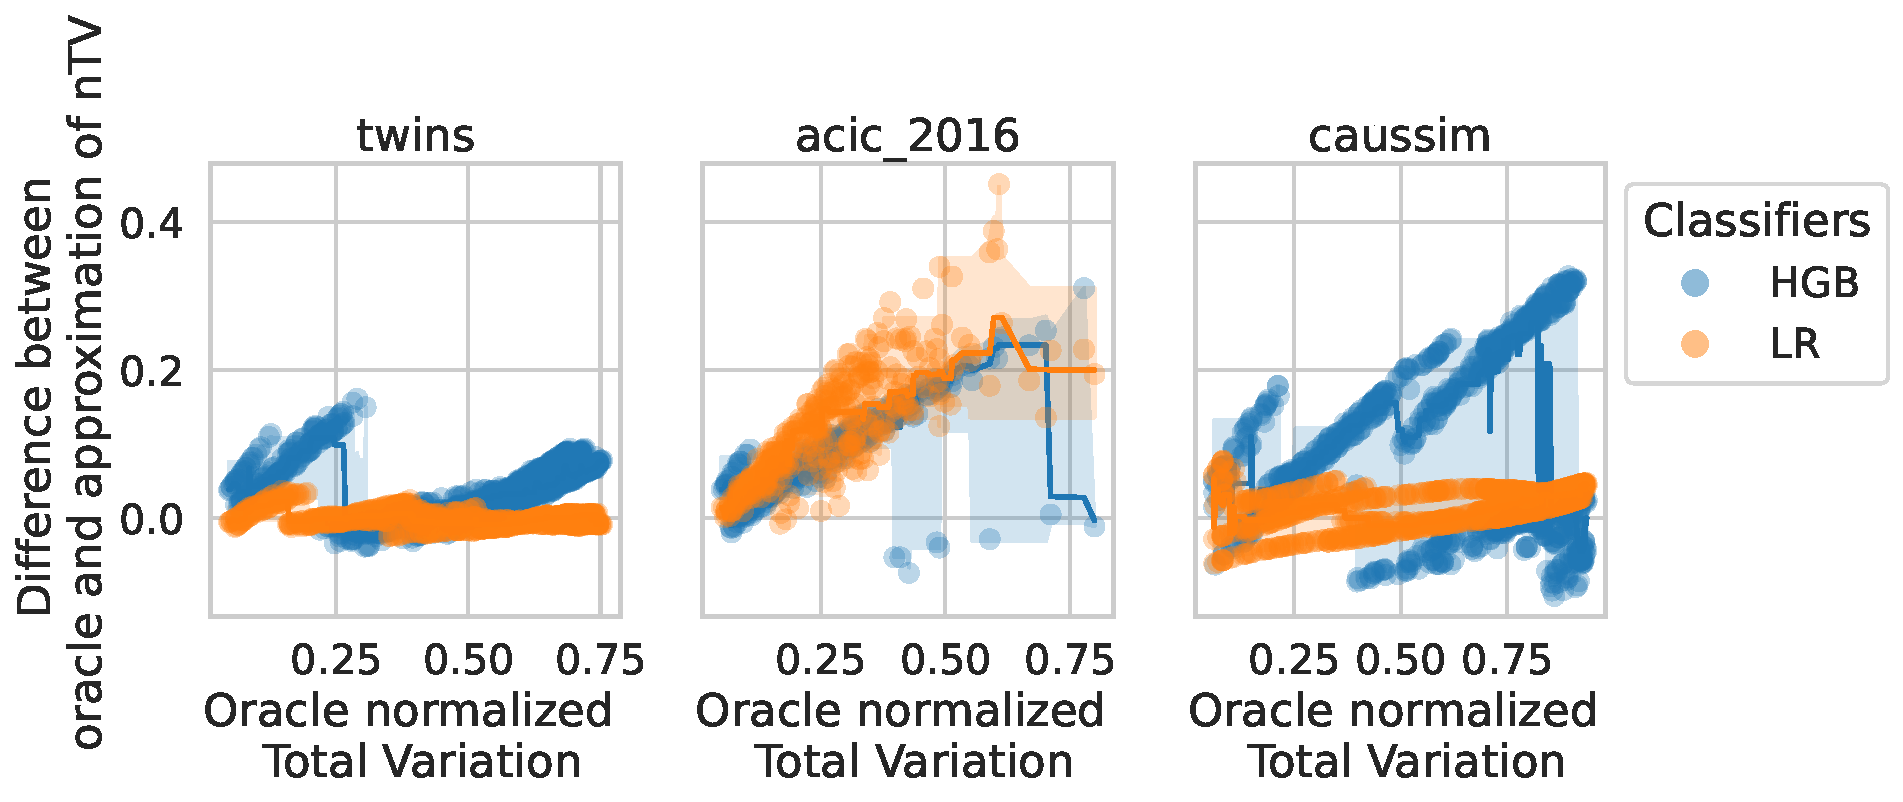
\includegraphics[width=\linewidth]{../img/chapter_5/overlap_measure_diff_oracle_ntv_to_n_tv_calibration=False_vs_oracle_n_tv.pdf}
    \end{subfigure}
    \begin{subfigure}[b]{\textwidth}
      \centering
      \caption{\textbf{Calibrated
          classifiers}}
      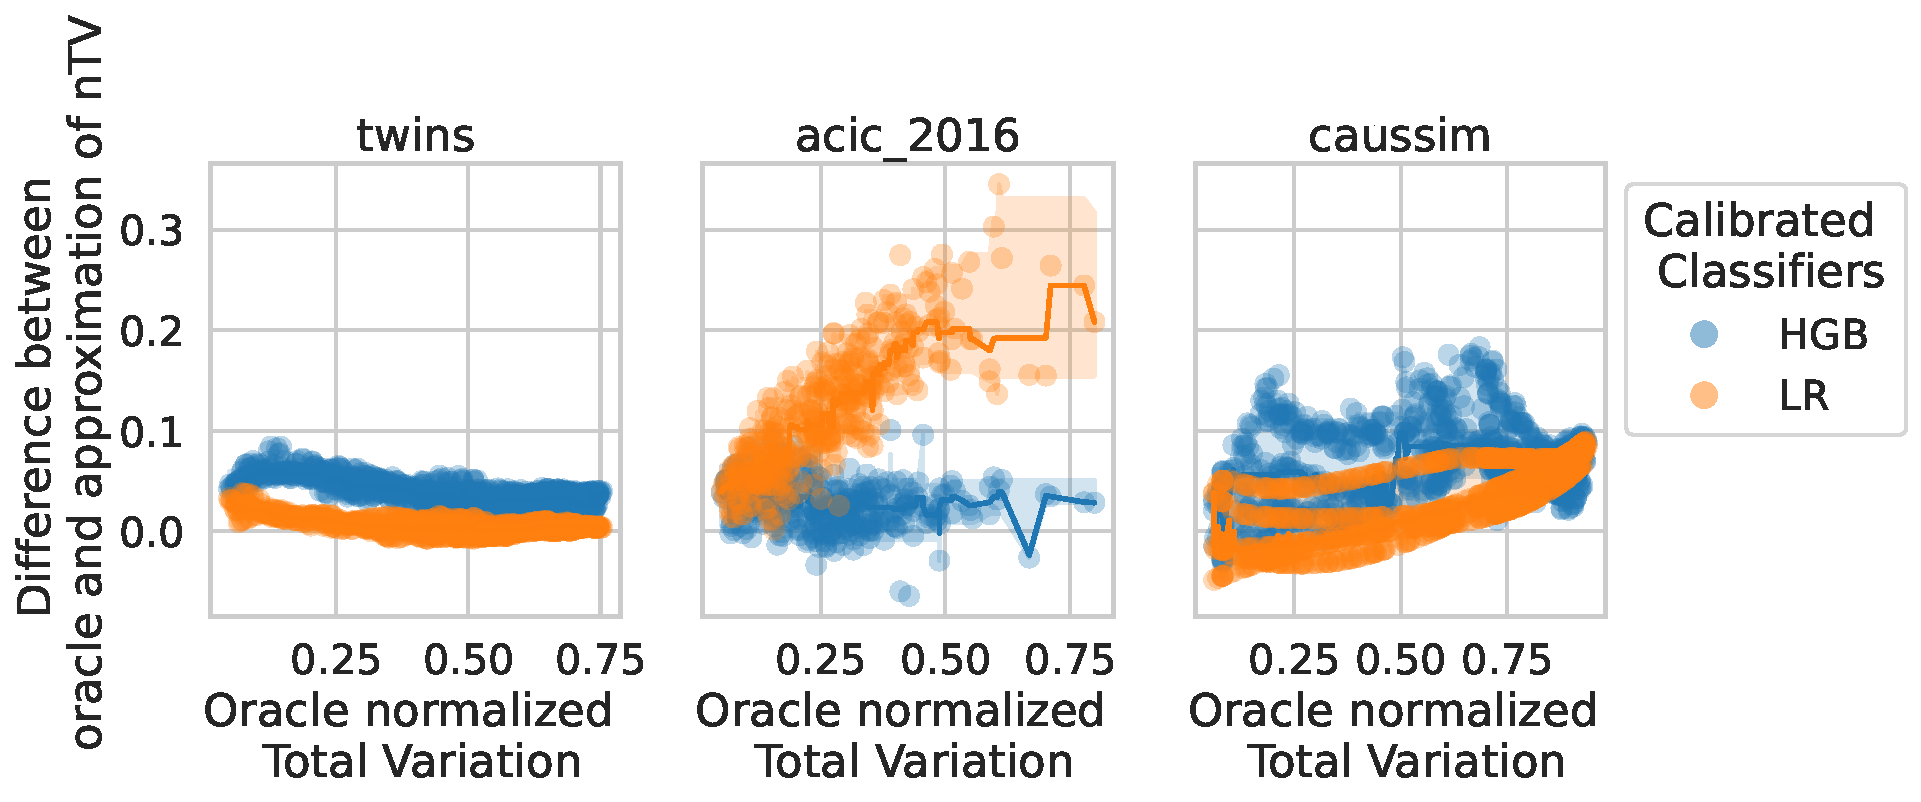
\includegraphics[width=\linewidth]{../img/chapter_5/overlap_measure_diff_oracle_ntv_to_n_tv_calibration=True_vs_oracle_n_tv.pdf}
    \end{subfigure}
    \caption{a) Without calibration, estimation of NTV is not trivial even for
      boosting models. b) Calibrated classifiers are able to recover the true
      Normalized Total Variation for all datasets where it is
      available.}\label{apd:overlap:ntv_approximation}
  \end{figure}

\end{appendices}





%%%%%%%%%%%%%%%%%%%%%%%%%%%%%%%%%%%%%%%%%%%%%%%%%%%%%%%%%%%%%%%
% 4eme de couverture
\ifthispageodd{\newpage\thispagestyle{empty}\null\newpage}{}
\thispagestyle{empty}
\newgeometry{top=1.5cm, bottom=1.25cm, left=2cm, right=2cm}
\fontfamily{rm}\selectfont

\lhead{}
\rhead{}
\rfoot{}
\cfoot{}
\lfoot{}

\noindent
%*****************************************************
%***** LOGO DE L'ED À CHANGER IMPÉRATIVEMENT *********
%*****************************************************

\includegraphics[height=2.45cm]{../img/EOBE}
\vspace{1cm}
%*****************************************************
\fontfamily{cmss}\fontseries{m}\selectfont

\small

\begin{mdframed}[linecolor=Prune,linewidth=1]

  \textbf{Titre:} Titre de la thèse en français


  \noindent \textbf{Mots clés:} Quelques mots-clé

  \vspace{-.5cm}
  \begin{multicols}{2}
    \noindent \textbf{Résumé:}Blabla
  \end{multicols}

\end{mdframed}

\begin{mdframed}[linecolor=Prune,linewidth=1]

  \textbf{Title:} Thesis title in English

  \noindent \textbf{Keywords:} Some keywords

  \begin{multicols}{2}
    \noindent \textbf{Abstract:} Blabla
  \end{multicols}
\end{mdframed}

%************************************
\vspace{\fill} % ALIGNER EN BAS DE PAGE
%************************************

\noindent
\color{Prune} \footnotesize Maison du doctorat de Université Paris-Saclay\\
2$^{\mathrm{e}}$ étage, aile ouest, École normale supérieure Paris-Saclay\\
4 avenue des Sciencs\\
91190 Gif-sur-Yvette, France
\end{document}
